\begin{figure}[htbp]

\begin{center}
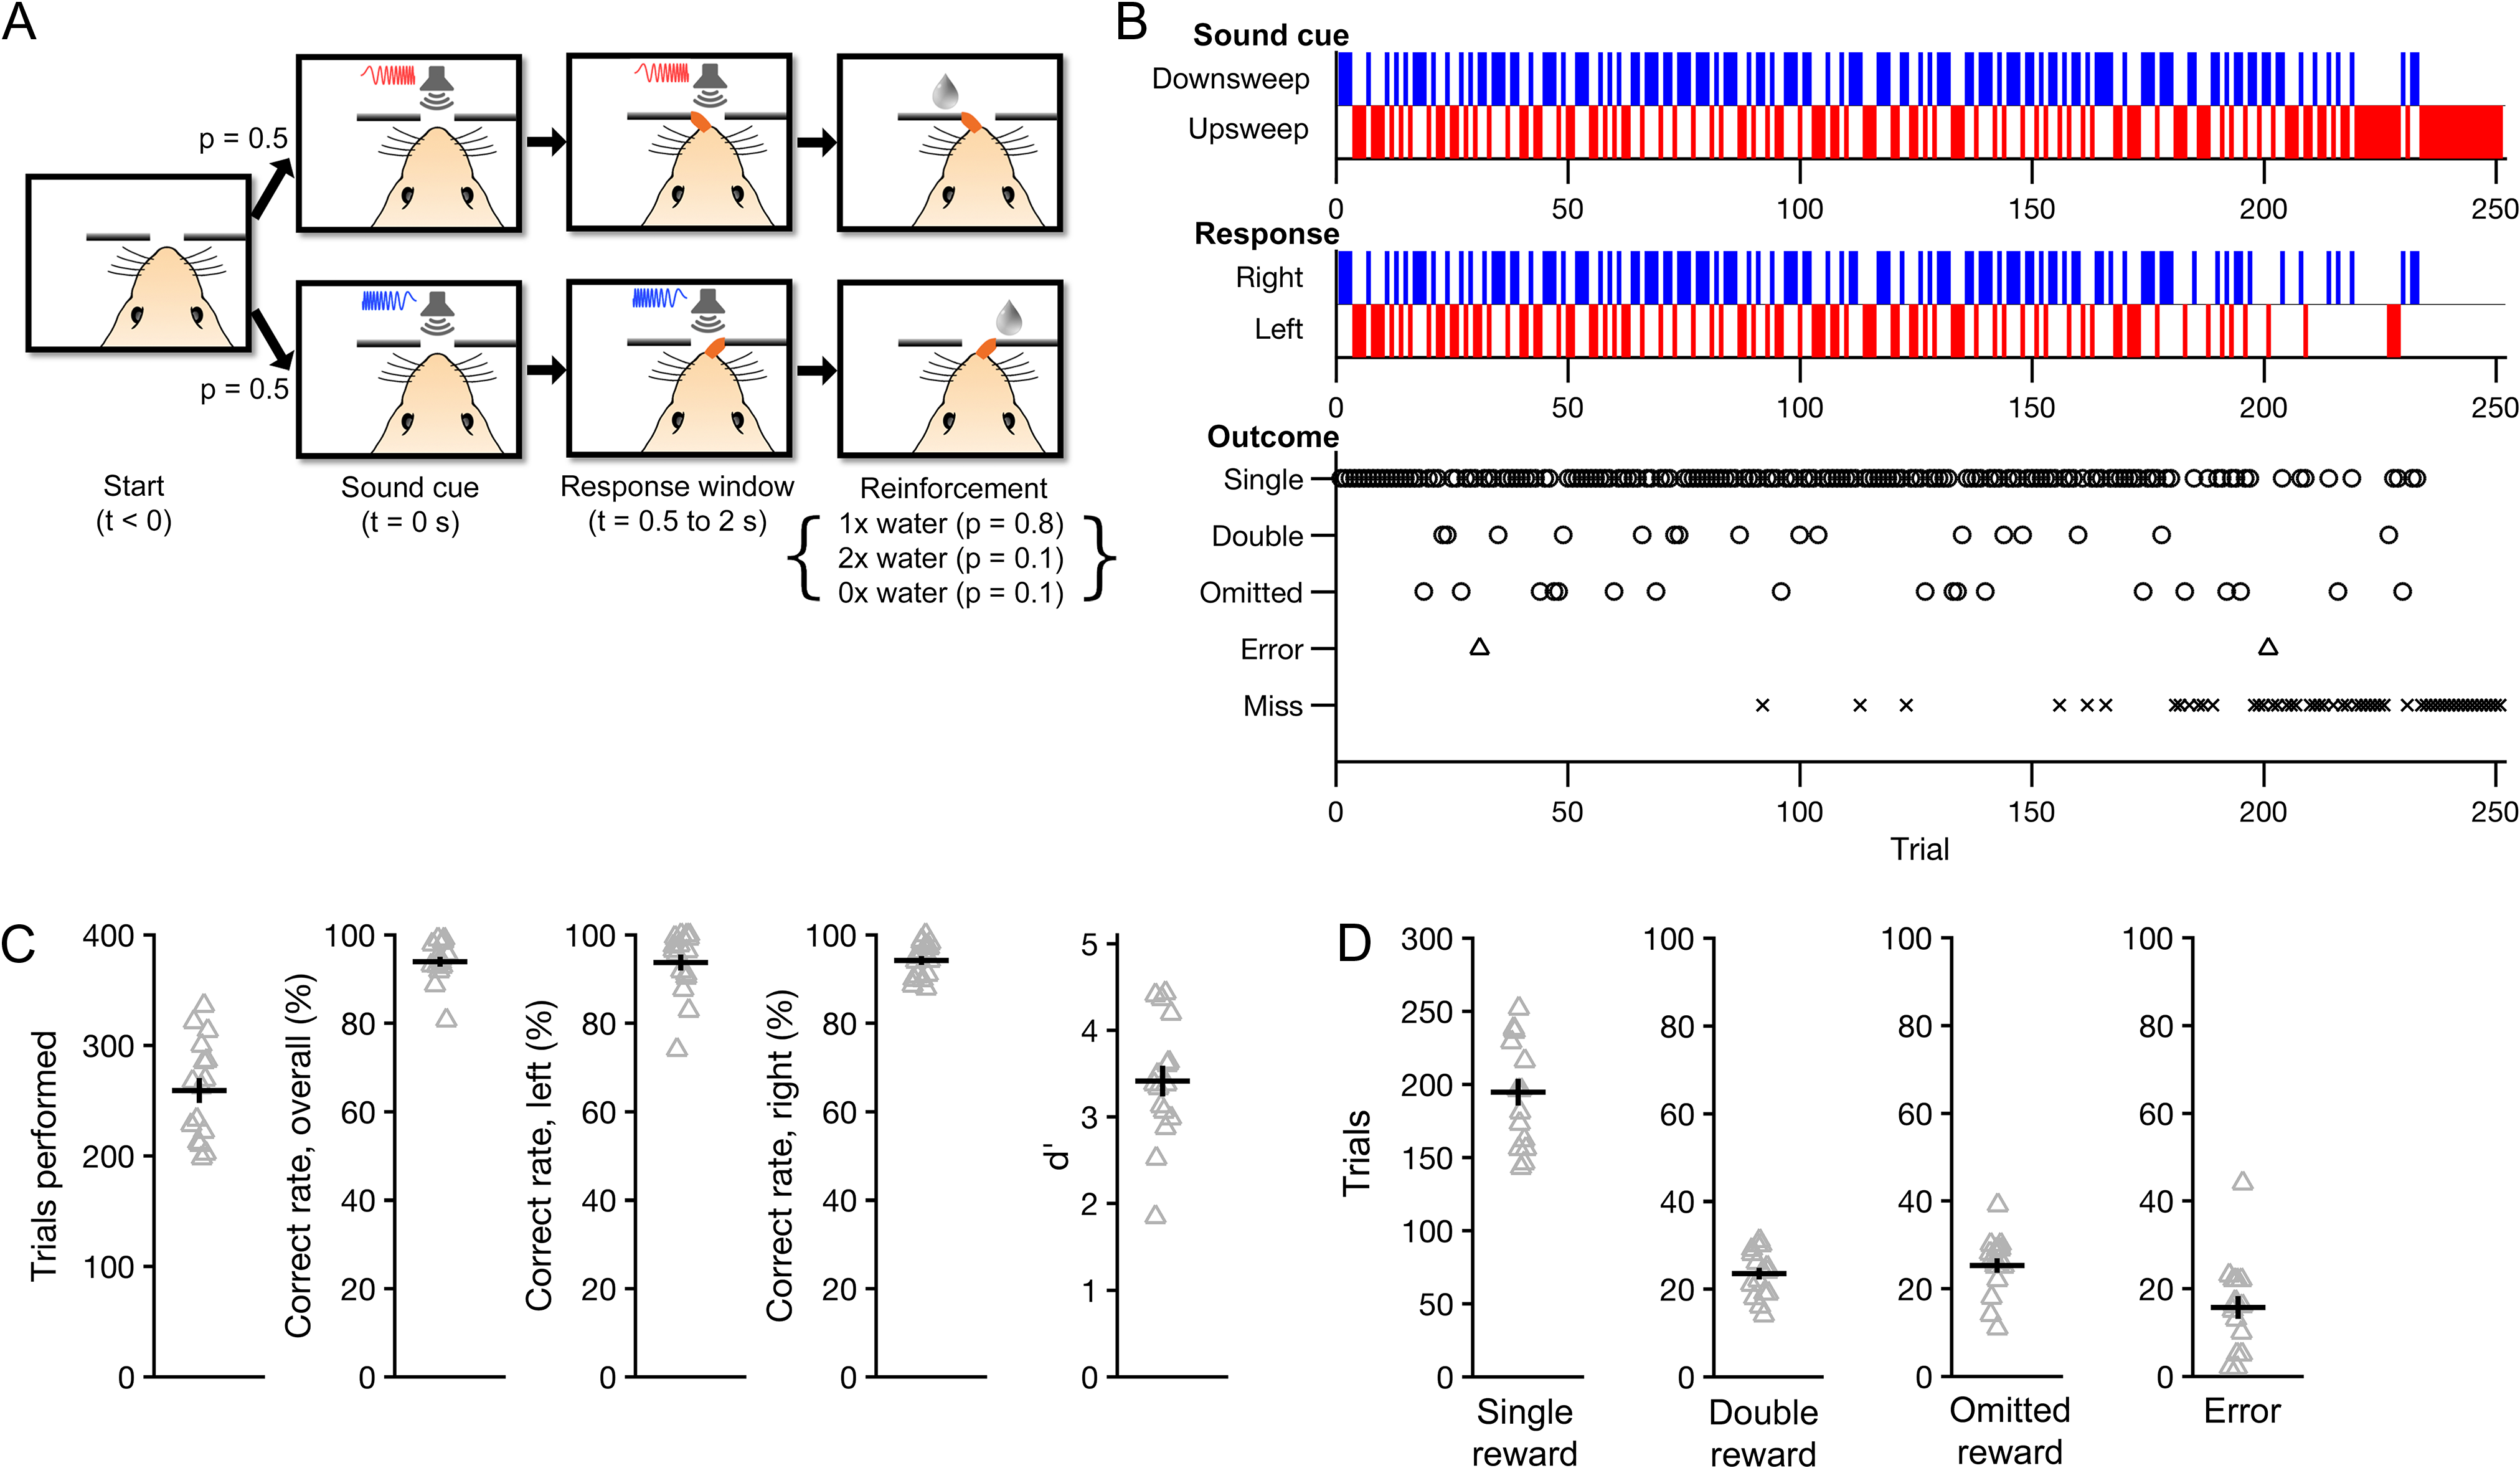
\includegraphics[width=\textwidth]{Figures/CC_fig1.png} 
\end{center}

\caption[Two-choice auditory discrimination task with probabilistic outcomes.]
{Two-choice auditory discrimination task with probabilistic outcomes. On each trial, mice were required to lick the target spout (left or right) indicated by a sound cue (upsweep or downsweep, respectively). Correct responses were rewarded probabilistically with one of three water amounts. (A) Flow diagram of the trial structure on correct trials. Each trial began with one of the two sound cues. The first lick to the target spout within 0.5–2 s following cue onset (Response window) immediately triggered one of three outcomes (Reinforcement): single reward ($1\times$), double reward ($2\times$) or omitted reward ($0\times$), with probabilities 80, 10 and 10\%, respectively. The next trial would begin 7 s after cue offset. (B) Behavioral performance from an example session (Experiment 1 in Table \ref{tab:CC_table1}). Occurrences of each sound cue (top), choice (middle) and outcome (bottom) are displayed in raster form according to trial number. Errors occurred when the non-target spout was chosen for the first lick within the response window. Misses were defined by the failure to respond within the response window. (C) Summary of behavioral performance. Gray triangles, individual sessions. Black cross-hairs, $mean \pm SEM$. (D) Number of occurrences of each outcome per session. For all figures, $N = 16$ sessions from 10 mice unless otherwise noted.}

\label{fig:CC_fig1}
\end{figure}
